\documentclass{article}

\usepackage{arxiv}

\usepackage[utf8]{inputenc} % allow utf-8 input
\usepackage[T1]{fontenc}    % use 8-bit T1 fonts
\usepackage{hyperref}       % hyperlinks
\usepackage{url}            % simple URL typesetting
\usepackage{booktabs}       % professional-quality tables
\usepackage{amsfonts}       % blackboard math symbols
\usepackage{nicefrac}       % compact symbols for 1/2, etc.
\usepackage{microtype}      % microtypography
\usepackage{graphicx}
\usepackage{float}
\usepackage{amsmath}
\graphicspath{ {./images/} }

\title{iSEE-tRNA: An Integrated Web Server for Generation, Evaluation, and Visualization of Engineered sup-tRNA}

\author{
 Zhuo Ouyang \\
  School of Life Science\\
  Sun Yat-sen University\\
  Guangzhou, PA 510275 \\
  \texttt{ouyzh25@mail2.sysu.edu.cn} \\
   \And
 Lingling Zheng \\
  College of Agriculture and Biotechnology\\
  Sun Yat-sen University\\
  Shenzhen, PA 518107 \\
  \texttt{zhengll33@mail.sysu.edu.cn} \\
  \And
%  Qiuhui Wu \\
%  College of Agriculture and Biotechnology\\
%  Sun Yat-sen University\\
%  Shenzhen, PA 518107 \\
%   \texttt{wuqh29@mail2.sysu.edu.cn} \\
}

\begin{document}
\maketitle
\begin{abstract}
    iSEE-tRNA is a comprehensive web server designed to address the challenges associated with the generation, evaluation, and visualization of engineered suppressor tRNAs (sup-tRNAs) for decoding stop codons. Suppressor tRNAs are a promising strategy for correcting nonsense mutations linked to various diseases, but current methods such as random mutagenesis and anticodon modification are time-consuming and cost-prohibitive. iSEE-tRNA offers an integrated solution by providing an AI-powered tRNA generation system that utilizes literature and database-derived data, coupled with the RFamGen algorithm to automatically generate novel sup-tRNA sequences tailored for stop codon decoding. The platform ensures multi-dimensional evaluation based on key criteria such as stop codon recognition, proper folding, identity element presence, and interaction with release factors, guaranteeing the functionality of engineered sup-tRNAs. Additionally, iSEE-tRNA incorporates intuitive visualization tools powered by R2DT and AlphaFold3, allowing users to inspect and refine their tRNA designs easily. By streamlining the process of sup-tRNA engineering and enabling systematic evaluation and visualization, iSEE-tRNA accelerates research in tRNA therapeutics and genetic code expansion, providing an accessible and cost-effective solution for the design and analysis of sup-tRNAs.
    \end{abstract}

\section{Introduction}
Suppressor tRNAs (sup-tRNAs) have emerged as a promising tool for correcting nonsense mutations associated with various genetic disorders \cite{albers_engineered_2023}. These mutations, caused by premature stop codons, can result in the loss of functional proteins, making sup-tRNAs a key therapeutic strategy to restore protein synthesis by decoding these stop codons. The design and application of sup-tRNAs, however, are hindered by the time-consuming and costly nature of traditional methods such as random mutagenesis and anticodon modification. Moreover, these approaches often lack systematic evaluation frameworks and accessible visualization tools, which are essential for optimizing and refining sup-tRNA designs.

To address these challenges, we developed iSEE-tRNA, an integrated web server designed to streamline the generation, evaluation, and visualization of engineered sup-tRNAs. By incorporating artificial intelligence (AI)-based tRNA generation, iSEE-tRNA leverages curated datasets of natural and engineered sup-tRNAs, utilizing the RFamGen algorithm to automatically generate novel tRNA sequences capable of decoding stop codons \cite{sumi_deep_2024}. Furthermore, the platform provides a multi-dimensional evaluation pipeline that ensures the functional success of sup-tRNAs by assessing key criteria such as stop codon recognition, structural integrity, identity elements for aminoacylation, and interaction with elongation factors. This systematic evaluation process guarantees that the generated sup-tRNAs meet the necessary requirements for effective translation.

In addition to these features, iSEE-tRNA offers an intuitive visualization interface powered by advanced tools like R2DT and AlphaFold3, allowing researchers to visualize and refine the secondary and tertiary structures of their engineered tRNAs. This user-friendly visualization aids in the validation of tRNA designs, enabling researchers to optimize their sequences before experimental implementation. Overall, iSEE-tRNA provides a comprehensive and accessible solution for the efficient design of sup-tRNAs, reducing both time and cost, while enhancing the accuracy and applicability of sup-tRNA engineering in genetic code expansion and tRNA therapeutics \cite{tang_recent_2022, shandell_genetic_2021}.




\section{MATERIALS AND METHODS}
\subsection{Data Acquisition and Download}

The data for this study was acquired from the Genomic tRNA Database (GtRNAdb), which provides comprehensive tRNA information across various organisms. In particular, the focus was on the collection of suppressor tRNAs (sup-tRNAs) designed to decode premature termination codons (PTCs), which are crucial for correcting nonsense mutations in genetic research. The sup-tRNAs examined in this study are specific to the CUA, UCA, and UUA stop codons, representing 644, 1968, and 205 sequences, respectively.

The acquisition process involved constructing URLs based on identifiers from a provided CSV file containing GenomeID and GtRNAdbID for each relevant tRNA. From these URLs, genomic sequences, secondary structures, and predicted mature tRNA sequences were extracted and recorded for each sup-tRNA. The data was then organized and saved in both CSV and FASTA formats for subsequent analysis.

By automating the data collection, we efficiently gathered the necessary tRNA information, which forms the basis of the analysis and supports further research in the field of genetic code expansion and tRNA-based therapeutics.

\begin{figure}[H]
    \centering
    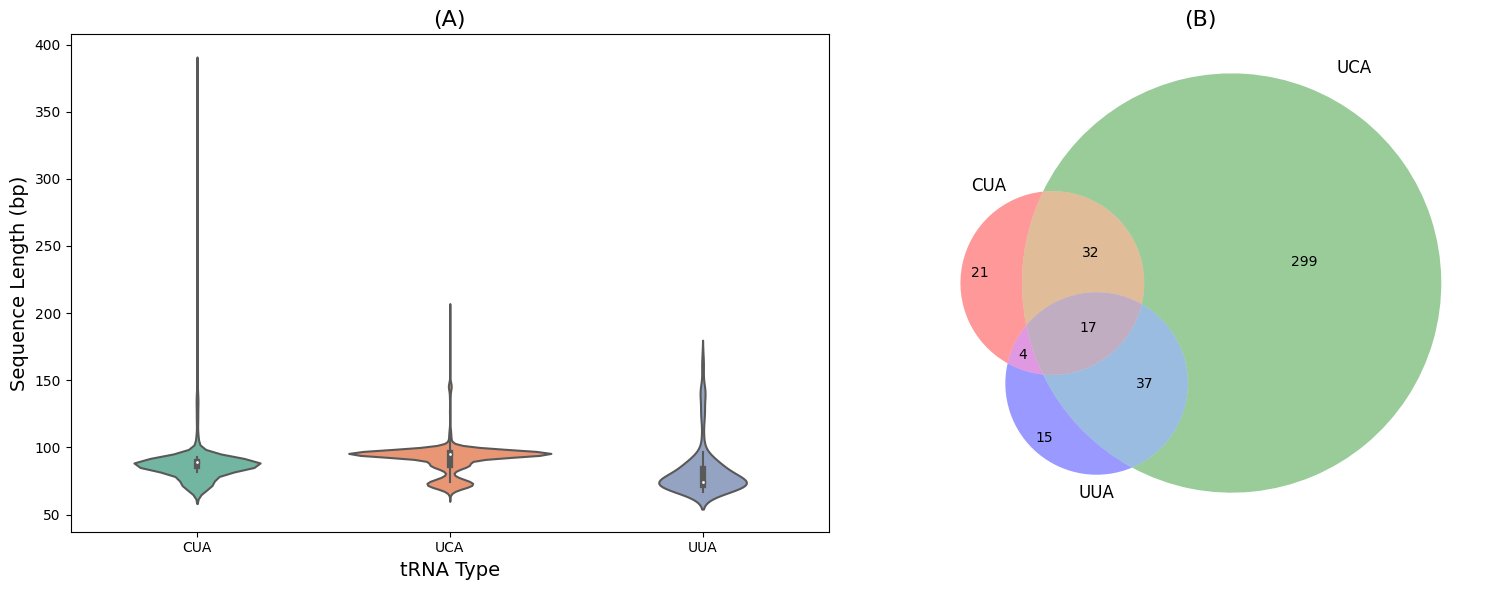
\includegraphics[width=\textwidth]{images/tRNATypes.png}
    \caption{(A) Sequence Length Distribution by tRNA Type. (B) Venn Diagram of Species Overlap.}
    \label{fig:tRNA_types}
\end{figure}

\subsection{Custom sup-tRNA Generator}

The Sequence Generator is based on the Variational Autoencoder (VAE) model \texttt{RFamgen}, utilizing artificial intelligence to generate a batch of candidate sup-tRNAs that meet user-defined requirements. Through deep generative models and reference datasets, iSEE-tRNA generates specific sup-tRNAs that satisfy user-selected criteria.

Users can select the target organism type, including Eukaryota, Prokaryota, and Archaea. Depending on the selected organism type, the generator uses the corresponding reference database to generate sup-tRNAs that match the biological characteristics of that type. Users can also customize the number of sequences to generate, with options such as 10, 50, 100, 500, or 1000 sequences, allowing for flexible experimentation.

The sequence generation process utilizes the \texttt{RFamgen} model, which is a VAE-based generative model capable of producing specific tRNA sequences based on user input. The generated tRNA sequences not only meet biological requirements but also provide high-quality prediction accuracy, making them suitable for genomic research, genetic code expansion, and tRNA-related therapeutic studies.

Through a simple user interface, users can select the stop codon of interest and specify the desired number of sequences. Once the generation process is initiated, the system automatically generates sup-tRNA sequences that meet the user's specifications based on the defined parameters.

With this custom functionality, users can generate sup-tRNA sequences tailored to their specific needs, further supporting genetic research. Below is the operation diagram of the sequence generator, showing how to select parameters and initiate the generation process, as shown in Figure \ref{fig:custom_gen}. For more information, visit the online tool at \href{https://isee-trna.lumoxuan.cn/CodonGenerator}{isee-trna.lumoxuan.cn/CodonGenerator}.

\begin{figure}[H]
    \centering
    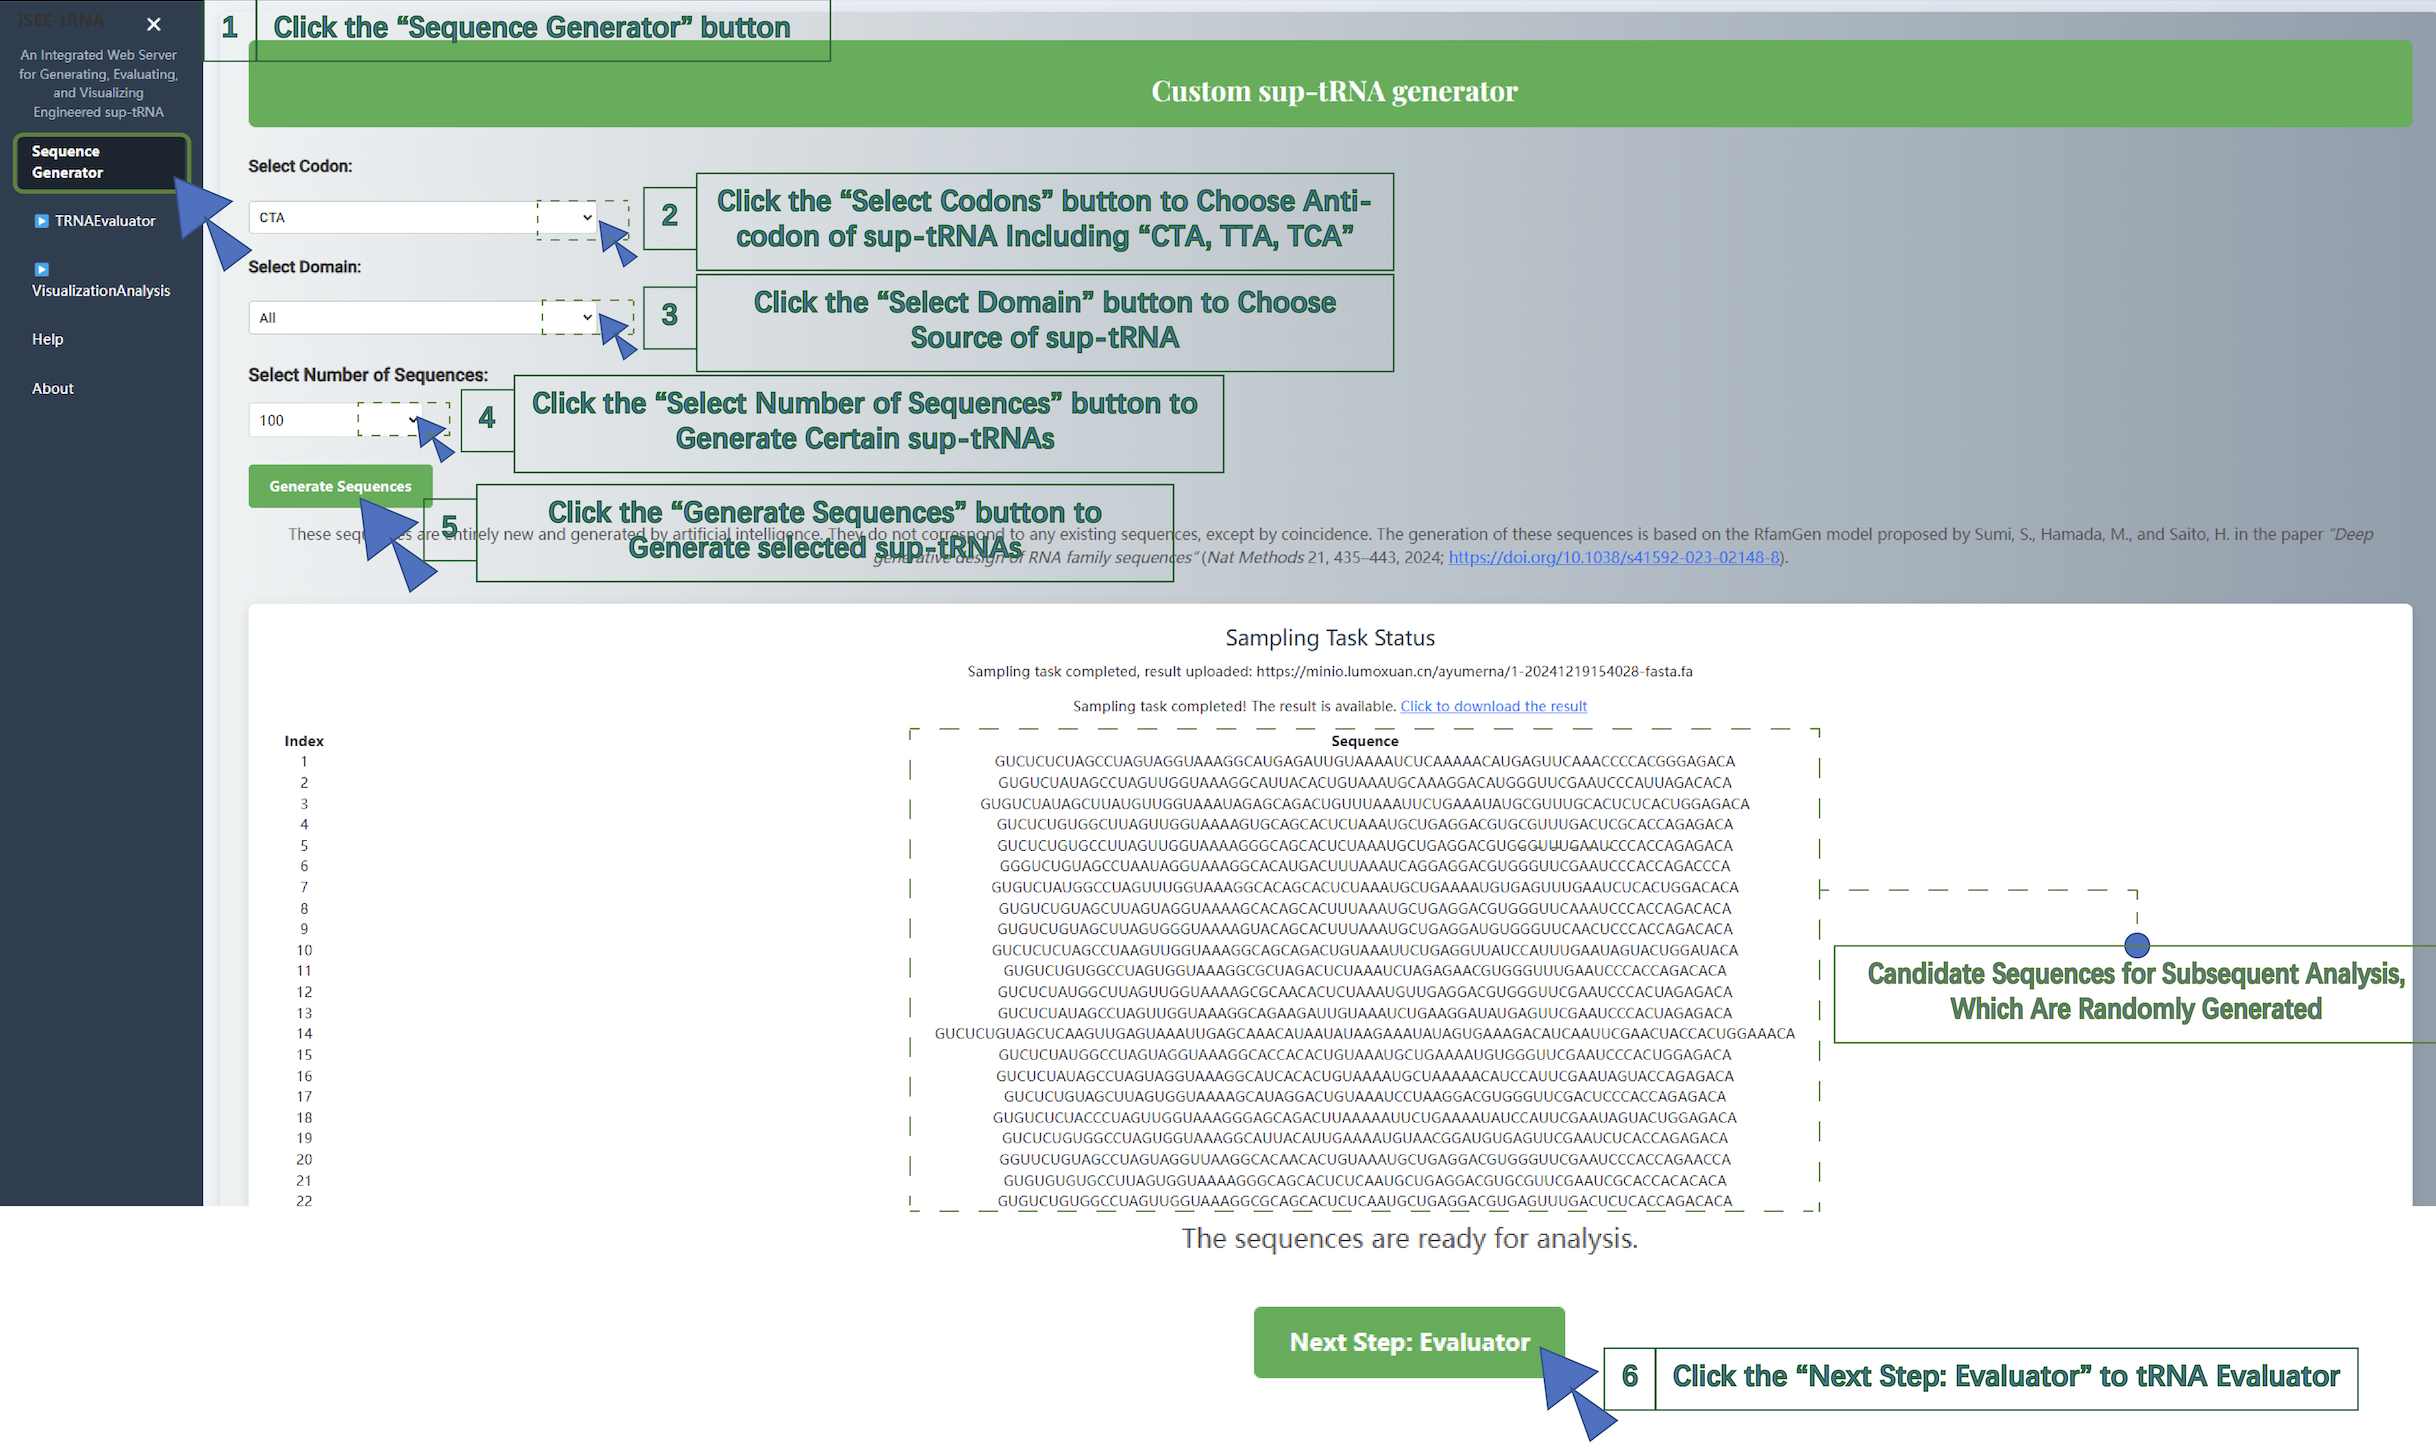
\includegraphics[width=\textwidth]{images/Custom}
    \caption{Operation diagram of the Sequence Generator: Select organism type, stop codon, and sequence quantity for generation.}
    \label{fig:custom_gen}
\end{figure}

\subsection{Structure Folding Evaluation}

In the process of evaluating sup-tRNA sequences, it is crucial to ensure that the generated tRNAs adopt the correct three-dimensional structure that is essential for their function. The Structure Folding Evaluation step in iSEE-tRNA uses the tool tRNAscan-SE to assess the folding of each tRNA sequence. This evaluation is essential because tRNAs must adopt a precise secondary and tertiary structure to be functional in translation, where they play a role in decoding mRNA codons into amino acids.

tRNAscan-SE is particularly useful in this step as it can predict the secondary structure of tRNAs by identifying conserved features such as the acceptor stem, D-loop, anticodon loop, and T-loop. These structural elements are vital for tRNA functionality, and any deviations from their typical folding patterns can impair the tRNA's ability to function correctly. By using tRNAscan-SE, the tool analyzes the sequences to determine whether the predicted folding matches the canonical tRNA structure, providing an infernal score that reflects the reliability and stability of the fold. A higher infernal score indicates that the tRNA sequence is likely to form a stable, functional structure.

The inclusion of tRNAscan-SE in the Structure Folding Evaluation step ensures that each generated sup-tRNA sequence not only matches the expected sequence properties but also adopts the correct structural configuration. This evaluation is critical for filtering out sequences that may be biologically irrelevant or unable to function properly in the context of genetic research or therapeutic applications. Moreover, the infernal score produced by tRNAscan-SE serves as a quantitative measure to compare the stability of different tRNA candidates, guiding researchers in selecting the most promising candidates for further study.

By using tRNAscan-SE in this evaluation step, the tool significantly enhances the accuracy of sup-tRNA predictions, ensuring that the generated sequences meet both sequence and structural requirements. After this evaluation, researchers can move on to further analyses, such as Identity Elements Evaluation, to confirm the functional compatibility of the sequences.


\subsection{Identity Elements Evaluation}

In this phase, the evaluation focuses on the identification and analysis of key identity elements in the RNA sequences, which are critical for determining the functional compatibility of the sequences as tRNAs. The identity elements typically include the\textbf{anticodon loop},\textbf{acceptor stem},\textbf{D-loop}, and\textbf{T-loop} regions of the tRNA. Each of these elements plays a crucial role in the interaction between the tRNA and its corresponding aminoacyl-tRNA synthetase or the ribosome during translation.

Let us define the sequence of a tRNA as \( S = (s_1, s_2, ..., s_n) \), where \( n \) is the length of the tRNA sequence. The identity elements \( I = (I_1, I_2, ..., I_m) \) are subsets of this sequence, corresponding to specific structural regions, where \( m \) is the number of identity elements identified.

For a given identity element \( I_k \), the position of each nucleotide \( s_i \) within \( I_k \) can be characterized by the following formula:

\[
P(I_k) = \{i : s_i \in I_k \}, \quad \textnormal{(where)} \quad 1 \leq i \leq n
\]

Where \( P(I_k) \) represents the set of positions in the tRNA sequence that belong to the identity element \( I_k \).

To evaluate the conservation of these elements across sequences, we define a score \( S_k \) for each identity element based on its conservation in a set of aligned tRNA sequences. Let \( A = (A_1, A_2, ..., A_m) \) be the set of aligned tRNA sequences, where each \( A_j \) is an aligned sequence from the dataset. The score for identity element \( I_k \) is given by:

\[
S_k = \frac{1}{|A|} \sum_{j=1}^{|A|} \mathbb{I}(P(I_k) \subset A_j)
\]

Where \( \mathbb{I}(P(I_k) \subset A_j) \) is an indicator function that returns 1 if the positions corresponding to \( I_k \) in sequence \( A_j \) match the expected positions in \( I_k \), and 0 otherwise.

The evaluation of identity elements also considers the conservation of the\textbf{anticodon}. The anticodon is defined as a sequence \( A_c \) that pairs with the codon in mRNA during translation. For a given sequence \( S \), the anticodon is located at positions \( P(A_c) \subset S \), and its conservation across sequences is measured by the following formula:

\[
C(A_c) = \frac{1}{|A|} \sum_{j=1}^{|A|} \mathbb{I}(P(A_c) \subset A_j)
\]

Where \( C(A_c) \) is the conservation score of the anticodon in the aligned sequences. A higher score indicates a more conserved anticodon sequence, which is crucial for the tRNA’s ability to recognize and bind to its corresponding codon.

Furthermore, for each identity element \( I_k \), we can compute a\textbf{conservation vector} \( V_k \), where each component of the vector corresponds to the conservation of the nucleotides at a specific position within the element. The vector is defined as:

\[
V_k = \left( v_{k1}, v_{k2}, ..., v_{km} \right)
\]

Where \( v_{ki} \) represents the conservation at position \( i \) within the identity element \( I_k \). The conservation at each position is calculated as:

\[
v_{ki} = \frac{1}{|A|} \sum_{j=1}^{|A|} \mathbb{I}(A_j[i] = s_i)
\]

Where \( A_j[i] \) is the nucleotide at position \( i \) in sequence \( A_j \), and \( s_i \) is the nucleotide at position \( i \) in the identity element \( I_k \).

This detailed analysis of identity elements ensures that the evaluated tRNAs not only have the correct sequence but also maintain the key structural features necessary for proper functionality. The conservation scores of these elements are used to identify the most promising tRNA candidates for further applications in genetic research or therapeutic development.

\[
\mathrm{Identity Elements Evaluation Score} = \sum_{k=1}^{m} S_k
\]

This final score aggregates the individual conservation scores of all identity elements, providing an overall measure of the tRNA's functional integrity.

\subsection{The affinity between aa-tRNAs and release factor}
The binding affinity between aminoacyl-tRNAs (aa-tRNAs) and elongation factor Tu (EF-Tu) is a critical factor in ensuring efficient delivery of tRNA during translation. For suppressor tRNAs (sup-tRNAs) designed to correct nonsense mutations, optimizing this affinity is essential to maintain translational fidelity and protein synthesis rates. Our computational pipeline addresses this challenge through systematic evaluation of tRNA structural features, with a focus on the T-stem region – a key determinant of EF-Tu binding energy.

\subsubsection{T-stem sequence optimization}
The T-stem (positions 49-51 and 63-65 in tRNA) contributes significantly to the thermodynamic stability of the tRNA-EF-Tu complex. Experimental studies have established that specific base pair combinations in this region exhibit distinct free energy contributions ($\Delta\Delta G^{\circ}$). Our implementation utilizes an empirical thermodynamic model to predict binding energy based on T-stem sequence:

\[
\Delta G^{\circ}_{\text{tRNA}} = \sum_{i=49,50,51} \Delta\Delta G^{\circ}_{\text{pair}_i}
\]

where $\Delta\Delta G^{\circ}_{\text{pair}_i}$ values are derived from position-specific energy tables . This approach enables rapid screening of tRNA variants for optimal EF-Tu binding.

\subsubsection{Computational workflow integration}
The analysis pipeline combines secondary structure prediction with energy calculation:

\begin{enumerate}
    \item \textbf{tRNAscan-SE structural analysis}: Identifies T-stem coordinates through pattern matching of secondary structure elements (>>>...<<<)
    \item \textbf{Base pair extraction}: Isolates critical positions (49-51/63-65) from predicted structure
    \item \textbf{Energy calculation}: Applies position-specific $\Delta\Delta G^{\circ}$ values using:
\end{enumerate}



\subsubsection{Design optimization strategy}
The tool supports three key optimization approaches:

\begin{itemize}
    \item \textbf{T-stem engineering}: Guides base pair selection using energy tables to achieve target $\Delta G^{\circ}_{\text{tRNA}}$
    \item \textbf{Structural validation}: Verifies canonical tRNA folding through tRNAscan-SE's infernal score
    \item \textbf{Energy balancing}: Maintains optimal $\Delta G^{\circ}_{\text{total}}$ (-10 to -12 kcal/mol) by compensating for amino acid contributions
\end{itemize}



This integrated approach enables researchers to systematically engineer sup-tRNAs with balanced EF-Tu binding characteristics, combining AI-generated sequences with physics-based energy optimization. The web interface at \url{iseetma.lumoxuan.cn/CodonGenerator} implements these calculations in real-time, providing immediate feedback on design quality.

\section{RESULTS}
\input{sections/result}

\section{DISCUSSION AND CONCLUSIONS}
\input{sections/discussion}

\bibliographystyle{unsrt}  
\bibliography{references}  % External .bib file for references

\end{document}